\documentclass[xcolor={usenames, dvipsnames}]{beamer}
\usepackage{amsmath, amssymb}
\usepackage[export]{adjustbox}
\usepackage{tikz}
\usepackage{wrapfig}
\usepackage{bm}
\usepackage{graphicx}

\mode<presentation> {
\usetheme{Singapore}
}

\title{\#1 Chad Allen Zhao gets the hottest girl in the grade}
\author{Ramesh Balaji, Duc Nguyen, Allen Zhao}
\date{June 11, 2021}

\begin{document}

\frame{\titlepage}

\begin{frame}
	It was the instant after the last game of senior year, and Allen Zhao—the number one basketball prospect coming from the Class of 2022—had absolutely crushed it, the other team making a total of 2 points the entire game. Allen was running outside in celebration and the entire school was chasing him. Of course, Allen, despite all the glory and victory, was only looking for one person in the crowd.
\end{frame}

\begin{frame}

    Allen Zhao and Tacko Fall go on a fast break with 20 seconds left on the game clock, in parallel
    motion $23 ft$ apart. 
Allen must pass it directly to Fall given that Allen is accelerating at ($0.5t^2+3)\frac{ft}{sec^2}$
with an initial velocity of $14 \frac{ft}{sec}$ and an initial position of 7 ft from the half-court and Fall is accelerating at ($0.6t^2+3t) \frac{ft}{sec^2}$
with an initial velocity of $18 \frac{ft}{sec}$ and an initial position of $12ft$ from the half-court. Allen throws the ball at 
$51 \frac{ft}{sec}$. Violet, watching the crowd has already calculated the answer to 
her challenge to Allen: to find $\frac{d\theta}{dt}$ when he throws the basketball at his
initial position. Now, Allen must do the same. 

\end{frame}

\begin{frame}
\frametitle{The Basketball Problem}

\begin{center}

    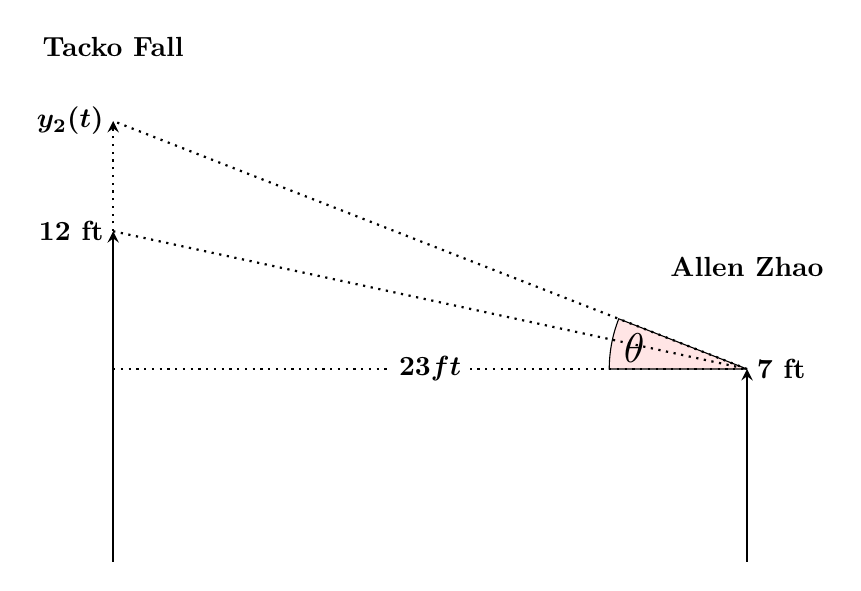
\begin{tikzpicture}[scale=0.35]
        \draw[fill=red!10] (23,1) -- (18,1) arc[start angle=180, end angle=158.629,radius=5cm] -- (23,1);
        %\draw[fill=red!20] (23,1) -- (15,1) arc[start angle=180, end angle=158.629,radius=8cm] -- (23,1);
        %\draw[fill=blue!20] (23,1) -- (17.25,1) arc[start angle=180, end angle=167.735,radius=5.75cm] -- (23,1);
        \draw[->, >=stealth, thick] (0,-6) -- (0, 6);
        \draw[->, >=stealth, thick][dotted] (0, 6) -- (0, 10);
        \draw[->, >=stealth, thick] (23, -6) -- (23,1);
        \draw[dotted, thick]
            (0,6) -- (23,1);
        \draw[dotted, thick]
            (0,1) -- (23,1);
        \draw[dotted, thick]
            (23,1) -- (0,10);
        \draw
            (23,1) node[anchor=west] {\textbf{7 ft}};
        \draw
            (0,6) node[anchor=east] {\textbf{12 ft}};
        \draw
            (0,10) node[anchor=east] {\bm{$y_{2}(t)$}};
        \draw
            (18,1.75) node[anchor=west][scale=1.5] {\textbf{$\theta$}};
        \draw 
            (0,12) node[anchor=south] {\textbf{Tacko Fall}};
        \draw 
            (23,4) node[anchor=south] {\textbf{Allen Zhao}};
        \node[fill=white] at (11.5,1) {\bm{$23 ft$}};
    \end{tikzpicture}

\end{center}

\end{frame}

\begin{frame}

    \centering

    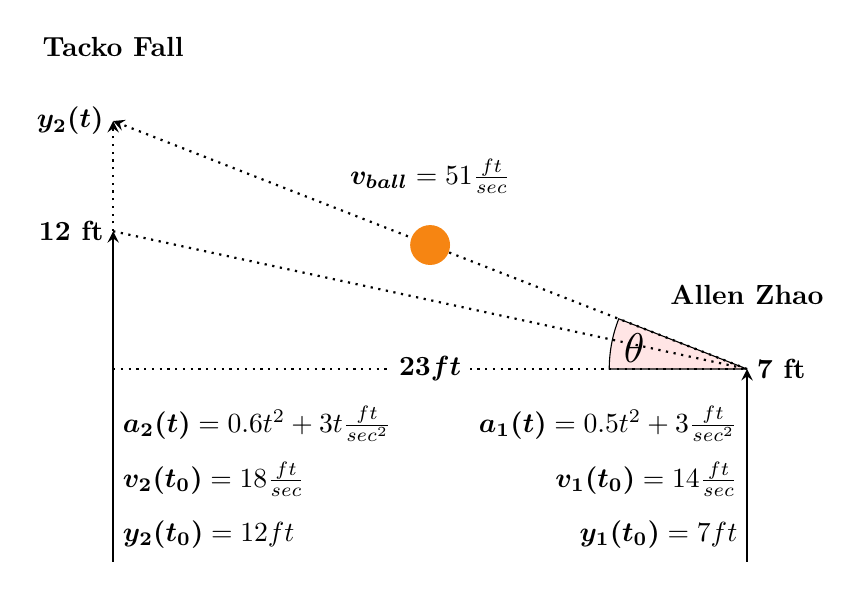
\begin{tikzpicture}[scale=0.35]
        \draw[fill=red!10] (23,1) -- (18,1) arc[start angle=180, end angle=158.629,radius=5cm] -- (23,1);
        %\draw[fill=red!20] (23,1) -- (15,1) arc[start angle=180, end angle=158.629,radius=8cm] -- (23,1);
        %\draw[fill=blue!20] (23,1) -- (17.25,1) arc[start angle=180, end angle=167.735,radius=5.75cm] -- (23,1);
        \draw[->, >=stealth, thick] (0,-6) -- (0, 6);
        \draw[->, >=stealth, thick][dotted] (0, 6) -- (0, 10);
        \draw[->, >=stealth, thick] (23, -6) -- (23,1);
        \draw[dotted, thick]
            (0,6) -- (23,1);
        \draw[dotted, thick]
            (0,1) -- (23,1);
        \draw[->, >=stealth, dotted, thick]
            (23,1) -- (0,10);
        \draw
            (23,1) node[anchor=west] {\textbf{7 ft}};

        \draw
            (0,6) node[anchor=east] {\textbf{12 ft}};
        \draw
            (0,10) node[anchor=east] {\bm{$y_{2}(t)$}};
        \draw
            (18,1.75) node[anchor=west][scale=1.5] {\textbf{$\theta$}};
        \draw 
            (0,12) node[anchor=south] {\textbf{Tacko Fall}};
        \draw 
            (23,3) node[anchor=south] {\textbf{Allen Zhao}};
        \draw
            (0,-1) node[anchor=west] {$\bm{a_{2}(t)} = 0.6t^2+3t \frac{ft}{sec^2}$};
        \draw
            (0,-3) node[anchor=west] {$\bm{v_{2}(t_{0})} = 18 \frac{ft}{sec}$};
        \draw
            (0,-5) node[anchor=west] {$\bm{y_{2}(t_{0})} = 12ft$};
        \draw
            (23, -1) node[anchor=east] {$\bm{a_{1}(t)} = 0.5t^2 + 3 \frac{ft}{sec^2}$};
            \draw
            (23, -3) node[anchor=east] {$\bm{v_{1}(t_0)} = 14 \frac{ft}{sec}$};
        \draw 
            (23, -5) node[anchor=east] {$\bm{y_{1}(t_0)} = 7 ft$};
        \draw
            (11.5, 7) node[anchor=south] {$\bm{v_{ball}} = 51 \frac{ft}{sec}$};
        \filldraw[color=BurntOrange] 
            (11.5, 5.5) circle (20pt);
        \node[fill=white] at (11.5,1) {\bm{$23 ft$}};
    \end{tikzpicture}\par

\end{frame}

\begin{frame}
    \centering
    \begin{figure}[t]
    
    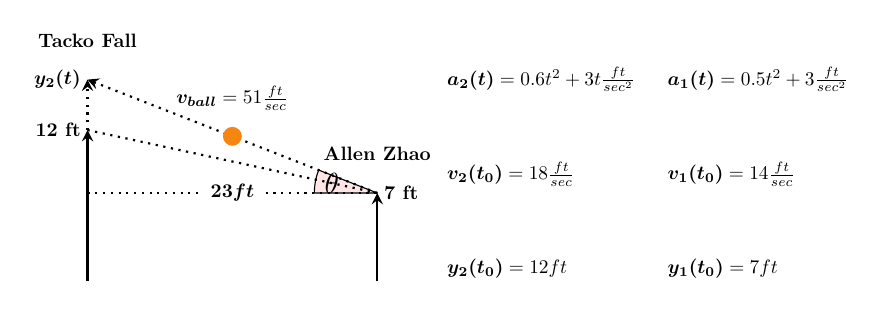
\begin{tikzpicture}[scale=0.16, every node/.style={scale=0.7}]
        \draw[fill=red!10] (23,1) -- (18,1) arc[start angle=180, end angle=158.629,radius=5cm] -- (23,1);
        %\draw[fill=red!20] (23,1) -- (15,1) arc[start angle=180, end angle=158.629,radius=8cm] -- (23,1);
        %\draw[fill=blue!20] (23,1) -- (17.25,1) arc[start angle=180, end angle=167.735,radius=5.75cm] -- (23,1);
        \draw[->, >=stealth, thick] (0,-6) -- (0, 6);
        \draw[->, >=stealth, thick][dotted] (0, 6) -- (0, 10);
        \draw[->, >=stealth, thick] (23, -6) -- (23,1);
        \draw[dotted, thick]
            (0,6) -- (23,1);
        \draw[dotted, thick]
            (0,1) -- (23,1);
        \draw[->, >=stealth, dotted, thick]
            (23,1) -- (0,10);
        \draw
            (23,1) node[anchor=west] {\textbf{7 ft}};

        \draw
            (0,6) node[anchor=east] {\textbf{12 ft}};
        \draw
            (0,10) node[anchor=east] {\bm{$y_{2}(t)$}};
        \draw
            (18,1.75) node[anchor=west][scale=1.5] {\textbf{$\theta$}};
        \draw 
            (0,12) node[anchor=south] {\textbf{Tacko Fall}};
        \draw 
            (23,3) node[anchor=south] {\textbf{Allen Zhao}};
        \draw
            (28,10) node[anchor=west] {$\bm{a_{2}(t)} = 0.6t^2+3t \frac{ft}{sec^2}$};
        \draw
            (28,2.5) node[anchor=west] {$\bm{v_{2}(t_{0})} = 18 \frac{ft}{sec}$};
        \draw
            (28,-5) node[anchor=west] {$\bm{y_{2}(t_{0})} = 12ft$};
        \draw
            (45.5, 10) node[anchor=west] {$\bm{a_{1}(t)} = 0.5t^2 + 3 \frac{ft}{sec^2}$};
        \draw
            (45.5, 2.5) node[anchor=west] {$\bm{v_{1}(t_0)} = 14 \frac{ft}{sec}$};
        \draw 
            (45.5, -5) node[anchor=west] {$\bm{y_{1}(t_0)} = 7 ft$};
        \draw
            (11.5, 7) node[anchor=south] {$\bm{v_{ball}} = 51 \frac{ft}{sec}$};
        \filldraw[color=BurntOrange] 
            (11.5, 5.5) circle (20pt);
        \node[fill=white] at (11.5,1) {\bm{$23 ft$}};
    \end{tikzpicture}\par

\end{figure}

Before Allen uses any of his given information on the motion of Fall and himself,
he should first look at the overarching equation for $\frac{d\theta}{dt}$.

    \begin{align*}
        tan(\theta) &= \frac{(12ft-7ft) + \Delta y_{2} ft}{23 ft} \\
        \theta &= tan^{-1}(\frac{5 + \Delta y_{2}}{23}) \\
        \frac{d\theta}{dt} &= \frac{1}{23} \cdot \frac{1}{1 + (\frac{5 + \Delta y_{2}}{23})^2} \cdot \frac{d(5 + \Delta y_{2})}{dt}
    \end{align*}

\end{frame}

\begin{frame}

    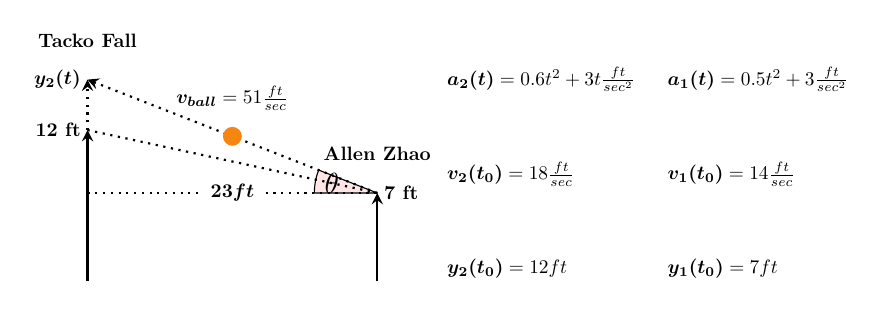
\begin{tikzpicture}[scale=0.16, every node/.style={scale=0.7}]
        \draw[fill=red!10] (23,1) -- (18,1) arc[start angle=180, end angle=158.629,radius=5cm] -- (23,1);
        %\draw[fill=red!20] (23,1) -- (15,1) arc[start angle=180, end angle=158.629,radius=8cm] -- (23,1);
        %\draw[fill=blue!20] (23,1) -- (17.25,1) arc[start angle=180, end angle=167.735,radius=5.75cm] -- (23,1);
        \draw[->, >=stealth, thick] (0,-6) -- (0, 6);
        \draw[->, >=stealth, thick][dotted] (0, 6) -- (0, 10);
        \draw[->, >=stealth, thick] (23, -6) -- (23,1);
        \draw[dotted, thick]
            (0,6) -- (23,1);
        \draw[dotted, thick]
            (0,1) -- (23,1);
        \draw[->, >=stealth, dotted, thick]
            (23,1) -- (0,10);
        \draw
            (23,1) node[anchor=west] {\textbf{7 ft}};

        \draw
            (0,6) node[anchor=east] {\textbf{12 ft}};
        \draw
            (0,10) node[anchor=east] {\bm{$y_{2}(t)$}};
        \draw
            (18,1.75) node[anchor=west][scale=1.5] {\textbf{$\theta$}};
        \draw 
            (0,12) node[anchor=south] {\textbf{Tacko Fall}};
        \draw 
            (23,3) node[anchor=south] {\textbf{Allen Zhao}};
        \draw
            (28,10) node[anchor=west] {$\bm{a_{2}(t)} = 0.6t^2+3t \frac{ft}{sec^2}$};
        \draw
            (28,2.5) node[anchor=west] {$\bm{v_{2}(t_{0})} = 18 \frac{ft}{sec}$};
        \draw
            (28,-5) node[anchor=west] {$\bm{y_{2}(t_{0})} = 12ft$};
        \draw
            (45.5, 10) node[anchor=west] {$\bm{a_{1}(t)} = 0.5t^2 + 3 \frac{ft}{sec^2}$};
        \draw
            (45.5, 2.5) node[anchor=west] {$\bm{v_{1}(t_0)} = 14 \frac{ft}{sec}$};
        \draw 
            (45.5, -5) node[anchor=west] {$\bm{y_{1}(t_0)} = 7 ft$};
        \draw
            (11.5, 7) node[anchor=south] {$\bm{v_{ball}} = 51 \frac{ft}{sec}$};
        \filldraw[color=BurntOrange] 
            (11.5, 5.5) circle (20pt);
        \node[fill=white] at (11.5,1) {\bm{$23 ft$}};
    \end{tikzpicture}\par

    \begin{align*}
        \frac{d\theta}{dt} = \frac{1}{23} \cdot \frac{1}{1 + (\frac{5 + \Delta y_{2}}{23})^2} \cdot \frac{d(5 + \Delta y_{2})}{dt}
    \end{align*}
    %
    Now, we need to solve for $\Delta y_2$. To do that, we need the time it takes for the ball to travel to Fall's future position. By Pythagoras, 
    %
    \begin{align*}
        (51 \cdot t_1)^2 = 23^2 + (5+\Delta y_2)^2
    \end{align*}

\end{frame}

\begin{frame}

    \begin{figure}[t]
        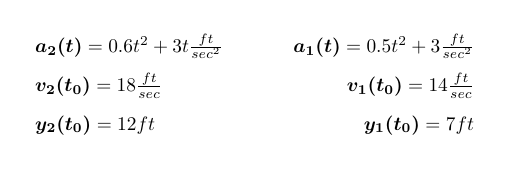
\begin{tikzpicture}[scale=0.25, every node/.style={scale=0.7}]
            \draw
                (0,-1) node[anchor=west] {$\bm{a_{2}(t)} = 0.6t^2+3t \frac{ft}{sec^2}$};
            \draw
                (0,-3) node[anchor=west] {$\bm{v_{2}(t_{0})} = 18 \frac{ft}{sec}$};
            \draw
                (0,-5) node[anchor=west] {$\bm{y_{2}(t_{0})} = 12ft$};
            \draw
                (23, -1) node[anchor=east] {$\bm{a_{1}(t)} = 0.5t^2 + 3 \frac{ft}{sec^2}$};
            \draw
                (23, -3) node[anchor=east] {$\bm{v_{1}(t_0)} = 14 \frac{ft}{sec}$};
            \draw 
                (23, -5) node[anchor=east] {$\bm{y_{1}(t_0)} = 7 ft$};
        \end{tikzpicture}
    \end{figure}

\vspace{-1cm}

    \begin{align*}
        (51 \cdot t_1)^2 = 23^2 + (5+\Delta y_2)^2
    \end{align*}

    Let's solve for $\Delta y_2$ and $t_1$. To do this, we will need to integrate $a_2(t)$, 
    then $v_2(t)$ given the initial positions and velocities. 
    %
    \begin{align*}
       \int_{0}^{t} (18\frac{ft}{sec}+\int_{0}^{t} (0.6t^2+3t) \ dt) \ dt &= \Delta y_2 \\
       \int_{0}^{t} (18\frac{ft}{sec}+\int_{0}^{t} (0.6t^2+3t) \ dt) \ dt &= \sqrt{(51t)^2 - 23^2} - 5 \\
       t = 0.535 sec, \Delta y_2 &= 9.718 ft
    \end{align*}

\end{frame}

\begin{frame}

    Now, we can finally solve for $\frac{d\theta}{dt} = \frac{1}{23} \cdot \frac{1}{1 + (\frac{5 + \Delta y_{2}}{23})^2} \cdot \frac{d(5 + \Delta y_{2})}{dt}$. 
    To find $\frac{d(5+\Delta y_2)}{dt}$, we need to use relative motion. The rate of change of that segment of the triangle would be:

    \begin{align*}
        18\frac{ft}{sec}+\int_{0}^{0.535}(0.6t^2+3t) \ dt = 18.461 \frac{ft}{sec}
    \end{align*}

    With everything plugged in:

    \begin{align*}
        \frac{d\theta}{dt} = \frac{1}{23} \cdot \frac{1}{1 + (\frac{14.718}{23})^2} \cdot 18.461 = 0.569 \frac{rad}{sec}
    \end{align*}

\end{frame}

\end{document}